\documentclass[letterpaper,11pt]{article}
\usepackage{amsmath,amssymb,bm} % input mathematics, \% -> %
\usepackage[hscale=0.8,vscale=0.8]{geometry} % set geometry of the paper
\usepackage{graphicx,setspace,listings} % insert graphs, determine line spacing, import text files

\begin{document}

\title{\textbf{Monte Carlo Simulation for a Brokerage House}} %\textbf -> bold font
\author{Chenyu Xu} % \textit -> italic, \\ -> new line
\date{\small June 12, 2015}

\maketitle
 
\begin{abstract}
Value at Risk (VaR) is a statistical technique used to quantify the level of financial risk within a firm or investment portfolio over a specific time frame.
In this final project, I perform a Monte Carlo simulation to calculate the VaR of the profit for each client in a brokerage house and the VaR of the total profit for the entire house.
In the simulation, the distribution and the correlations of the historical data of the stocks are preserved by implementing the resampling method.
\end{abstract}

\doublespacing

\section{Introduction and Setting}
One major responsibility of a brokerage house is to facilitate transactions between buyers and sellers as an intermediary in the financial market.
The primary job of a risk manager in a brokerage house is to ensure that market risks are not taken beyond the level at which the firm can take.
In this project, there is a brokerage house that has 100 clients trading 98 stocks every day. 
In order to estimate the market risk for all the clients and the entire brokerage house, we are asked to find out the Value at Risk (VaR) of the profits after trading for $N$ days in the future using a Monte Carlo simulation.
VaR is a measurement of profit or loss for a specific portfolio.
In our case, for a confidence level $p$, the VaR represents the maximal profit of a portfolio with probability $p$.

The basic assumptions for the simulation are the following.
For the $N$ days in the future, the clients remain the same position for the stocks they are holding.
The simulated future prices of the stocks are based on the 250-day historical data ending on March 31st, 2015, and they should reflect the same distribution (averages and volatility) and mutual correlations as the historical data.
$N$ and $p$ together with the clients' position data are the free parameters of the simulation.

During the simulation, two steps are particularly important.
First, we need to implement an algorithm so that the simulated stock prices reflect their historical correlations.
To do that, we can either use a random number generator based on correlated Gaussian model or directly resample the historical data.
In my simulation, I use the latter method because the resampling method does not assume any models for the distribution of the historical data.
Second, since we want to find out the VaR of profit for a portfolio, we need to first calculate the profit for this portfolio given each simulation scenario, and then perform a VaR calculation using the profit data.

\section{Explanation of Codes}

Following the class materials, I use Python to perform the simulation. 
The codes begin with loading a few libraries, \texttt{nlib} for using its \texttt{YStock} and \texttt{PersistentDictionary} classes, \texttt{pickle} for importing the file containing the clients' position data, \texttt{sys} for enabling command line input of parameters, \texttt{datetime} for access to the standard date format, and \texttt{random} for generating necessary random numbers.
The remaining part of the codes is dedicated to the implementation of a few class functions that belong to the class \texttt{Broker} and the \texttt{main()} function that executes the simulation.

\texttt{get\_client\_data()} This class function loads the \texttt{pickle} file containing the clients' position data.
The client list, the stock list, and the clients' position data are separately saved as class variables.
In particular, the data corresponding to the stocks with erroneous ticker symbol BRK.B and WAG are removed using the minus and intersection operations belonging to the \texttt{set} type.

\texttt{get\_stock\_data()} This class function loads the stock data using the \texttt{historical()} function of the \texttt{YStock} class in the \texttt{nlib} library. 
Once imported, the data are also stored in the local drive using the \texttt{PersistentDictionary} class in the \texttt{nlib} library.
The last 250 records of historical log return and the adjusted close on March 31th of all the stocks are subsequently extracted as two dictionaries with ticker symbols as keys and saved as class variables.
Although not shown in the codes, I have separately checked that the 250 records for each stock correspond to the same 250 trading days.

\texttt{simulate\_once()} This class function returns the simulated future prices of the stocks on the $N$-th future day using the resampling method and the historical data.
To maintain the correlation between the stocks, a list of random days is first generated.
A simulated future trading day is simply a random day in the past.
Note that the return of this function is a list rather than a single number as implemented in the \texttt{MCEngine} class in the \texttt{nlib} library.

\texttt{simulate\_many()} This class function calls \texttt{simulate\_once()} multiple times until the convergence condition is satisfied.
Since the return of \texttt{simulate\_once()} is a list, I define a number of dictionary variables (\texttt{results}, \texttt{s1}, \texttt{s2}, \texttt{mu}, and \texttt{dmu}) that can store all the simulation results and all the intermediate numbers needed to decide if the simulation is convergent.
The criterion of convergence is that the simulated stock prices of all the stocks are simultaneously convergent.
I use a counter (\texttt{flag}) to count the number of convergent stocks and compare it to the total number of stocks.

\texttt{quantile()} This function returns the quantile of list of numbers given a probability or confidence level. 
The input list is fed into the function through the parameter \texttt{data}, which immediately receives a self copy so that the list does not get changed in the parent function that calls the \texttt{quantile()} function.

\texttt{print\_client\_var()} This function generates a list of profits for each customer and calls the \texttt{var} function to obtain and print out the VaR for each customer.
Given a simulation scenario, the profit of each customer is calculated as the difference between simulated future price and today's price,  multiplied by the number of shares the customer is holding, and finally summed over all the stocks.

\texttt{print\_house\_var()} This function generates a list of profits for the whole brokerage house and calls the \texttt{var} function to obtain and print out the VaR for the house.
To obtain the total profit of the whole house given a simulation scenario, I first calculate the total number of shares for each stock and save it as a dictionary \texttt{n\_shares}.
The rest of the function is similar to \texttt{print\_client\_var()}.

\texttt{main()} This function is the execution part of the implemented \texttt{Broker} class.
A \texttt{Broker} object is generated, class variables are specified, and class functions are sequentially called to perform the Monte Carlo simulation and print out the results.

\section{Discussions}

In this simulation, I use the resampling method to generate the future log returns and the future prices for a given set of stocks because the correlated Gaussian model does not always provide a good description of the stock data.
For example, I make a quantile--quantile (Q--Q) plot of the historical log returns of Southern Company (SO) stock based on the past 250 trading days (Figure~\ref{fig:qqplot_SO}).
On the negative side, the SO log return data has quite a few points below the standard Gaussian distribution.
This indicates that the distribution of the log return data has a fatter tail than the Gaussian distribution.

\begin{figure}[h]
\centering
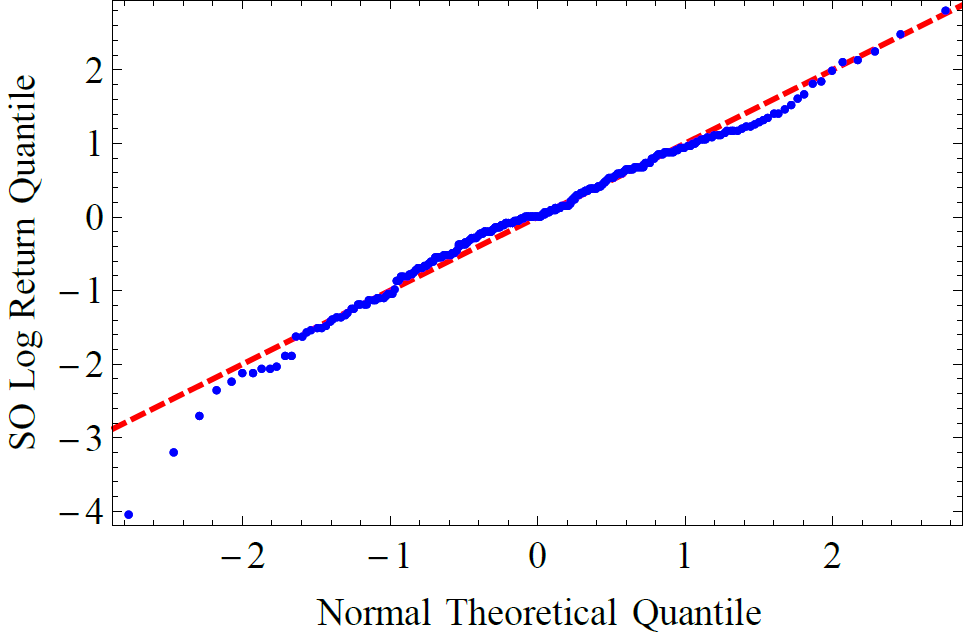
\includegraphics[width=0.49\textwidth]{qqplot_SO.png}
\caption{The Q--Q plot of the historical log returns of SO in the past 250 trading days.
The red dashed line ($y=x$) represents the ideal Gaussian distribution.}
\label{fig:qqplot_SO}
\end{figure}

To demonstrate that the resampling method preserves the correlation between stocks, I plot the correlations between SO and six selected stocks (Figure~\ref{fig:corr_SO}).
The historical correlations are calculated using the log returns of the past 250 trading days, while the future correlations are calculated using the resampling result of one trading day repeated by 250 times.
As can be seen in Figure~\ref{fig:corr_SO}, the historical correlations between SO and these six stocks span a large range between $-0.10$ and $0.85$.
The simulated future log returns are capable of reflecting these inherent correlations.

\begin{figure}[h]
\centering
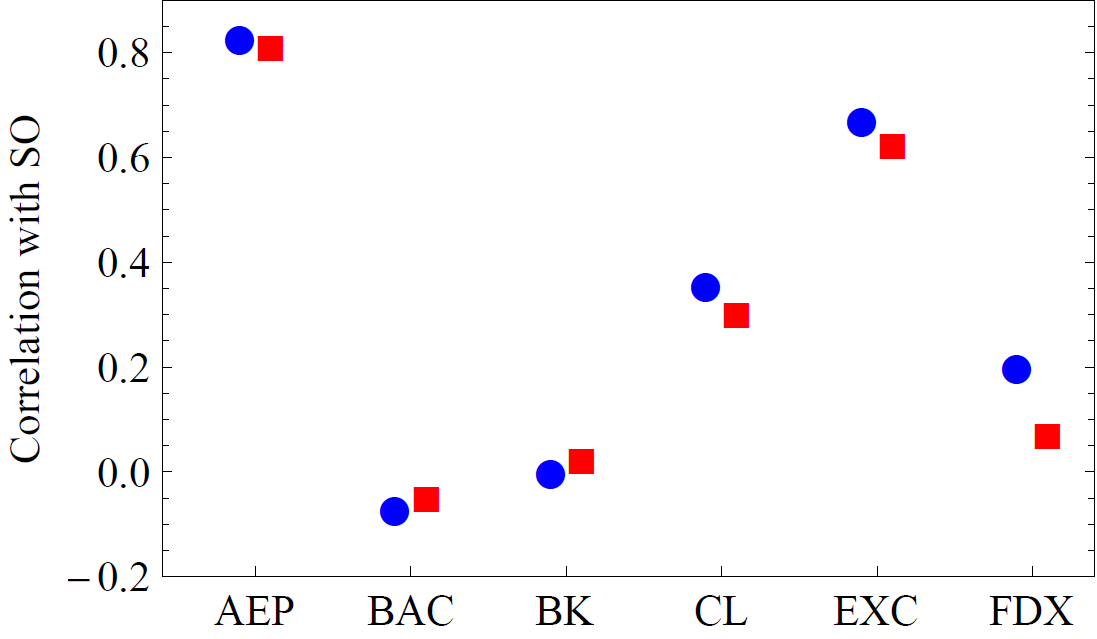
\includegraphics[width=0.49\textwidth]{corr_SO.png}
\caption{The correlations between SO and six other stocks, American Electric Power (AEP), Bank of America Corporation (BAC), The Bank of New York Mellon (BK), Colgate-Palmolive (CL), Exelon Corporation (EXC), and FedEx (FDX).
Historical correlations (blue circles) are calculated using the log returns of the past 250 trading days.
Future correlations (red squares) are calculated using the resampling result of one trading day repeated by 250 times.}
\label{fig:corr_SO}
\end{figure}

Once enough scenarios have been simulated, the correct procedure to obtain the VaR for the clients is to calculate the profit for each client given one scenario, then generate a list of profits corresponding to different scenarios, and finally calculate the VaR.
This is because there exists correlations between the prices of different stocks, as shown in Figure~\ref{fig:corr_SO}.
Note that the covariance between stock prices and that between log returns are related by
\begin{equation}
\text{cov}(S_1,S_2)=\text{cov}(S_1^0\text{e}^{R_1},S_2^0\text{e}^{R_1})\approx
S_1^0S_2^0\text{cov}(R_1,R_2)\quad\text{for } R_1,R_2\ll1,
\end{equation}
where $S_i$ is the stock price, $S_i^0$ is the initial stock price, and $R_i$ is the log return.
This leads to the correlation between the stocks $\text{corr}(S_1,S_2)=\text{corr}(R_1,R_2)$.
To visualize the correlations, I make an intensity plot of the correlations between all the stocks using their simulated prices (Figure~\ref{fig:corr_stocks}).
The correlation is peaked at $0.4$ and has a width of about $0.2$.
As a result, in calculating the VaR for a given client, it will give a wrong answer if one calculates the VaR for each stock first and then calculates the total VaR according to the client's portfolio.
For example, from the simulation result, I find that the wrong procedure gives \$57,421 for client.000, while the correct procedure gives only \$39,668.

\begin{figure}[h]
\centering
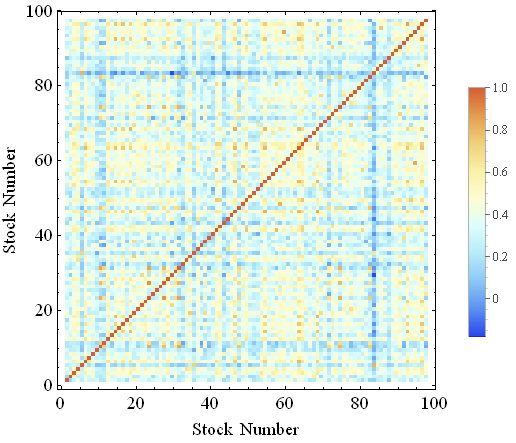
\includegraphics[width=0.49\textwidth]{corr_stocks.png}\ \ 
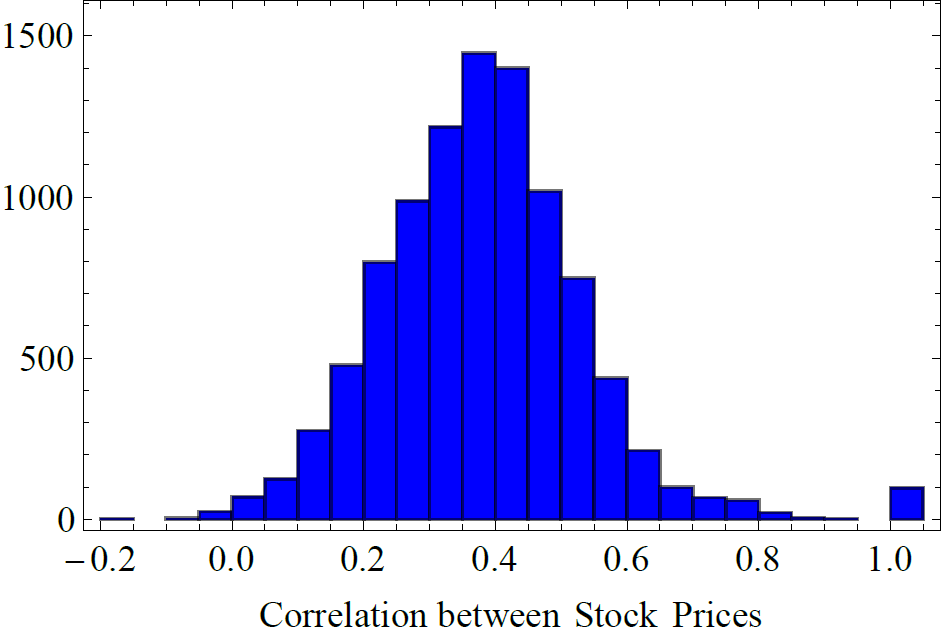
\includegraphics[width=0.45\textwidth]{hist_corr_stocks.png}
\caption{Left: the correlations between the prices of the stocks based on the resampling result of one trading day repeated by 250 times.
Right: the histogram of the correlations.}
\label{fig:corr_stocks}
\end{figure}

Similarly due to the correlations between the portfolios of different clients, I always calculate the total profit of the brokerage house given one scenario.
Suppose the portfolio of the $i$-th customer is $C_i=\sum_ma_{im}S_m$ where $C_i$ is the total net worth and $a_{im}$ is the number of share for the $m$-th stock held by the $i$-th client.
The covariance between the clients is $\text{cov}(C_1,C_2)=\sum_{m,n}a_{1m}a_{2n}\text{cov}(S_m,S_n)$.
Therefore the correlation between the clients is
\begin{equation}
\text{corr}(C_1,C_2)=\frac{\sum_{m,n}a_{1m}a_{2n}\text{cov}(S_m,S_n)}{\sqrt{\sum_{m,n}a_{1m}a_{1n}\text{cov}(S_m,S_n)}\sqrt{\sum_{m,n}a_{2m}a_{2n}\text{cov}(S_m,S_n)}},
\end{equation}
and is plotted (Figure~\ref{fig:corr_clients}).
The correlation is peaked at $0.94$ and has a width of about $0.08$.
Such a high correlation between clients implies that investors tend to choose similar investment portfolios given the same market environment.
One simulation result yields a VaR of \$6,934,454 for the brokerage house which is different from the sum of VaR's of all the clients \$7,329,131 due to the correlations.

\begin{figure}[h]
\centering
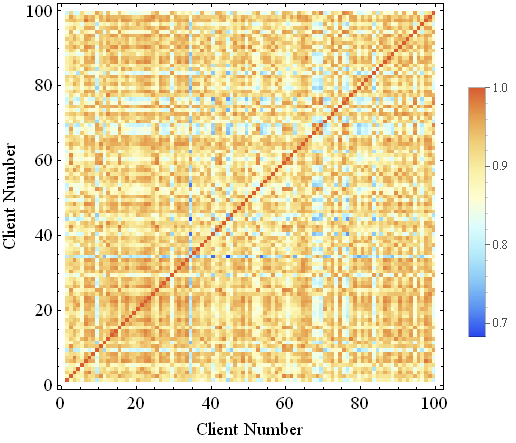
\includegraphics[width=0.49\textwidth]{corr_clients.png}\ \ 
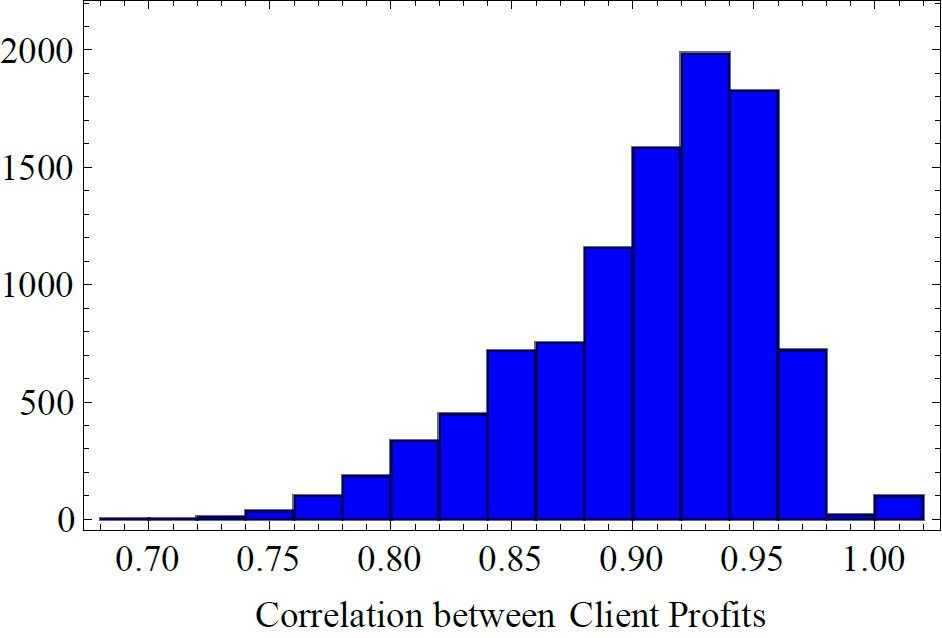
\includegraphics[width=0.45\textwidth]{hist_corr_clients.png}
\caption{Left: the correlations between the profits of the clients based on the resampling result of one trading day repeated by 250 times.
Right: the histogram of the correlations.}
\label{fig:corr_clients}
\end{figure}

\section{Conclusion}

I have performed a Monte Carlo simulation to calculate the VaR of the profit for each client in the brokerage house and the VaR of the total profit for the entire house.
The correlation of the simulated future stock prices are preserved by resampling the historical data of all the stocks on the same trading day.
Due to the inherent correlations, I always obtain one result given one simulation scenario and then calculate the VaR of a list of results corresponding to multiple scenarios.

\end{document}